%%%%%%%% ICML 2018 EXAMPLE LATEX SUBMISSION FILE %%%%%%%%%%%%%%%%%

\documentclass{article}

% Recommended, but optional, packages for figures and better typesetting:
\usepackage{amsmath, amssymb, amsthm}
\usepackage{mathtools}
\usepackage{microtype}
\usepackage{graphicx}
\usepackage{subfigure}
\usepackage{booktabs} % for professional tables
\usepackage{array}
\usepackage{xcolor}
\usepackage{algorithmic}

% hyperref makes hyperlinks in the resulting PDF.
% If your build breaks (sometimes temporarily if a hyperlink spans a page)
% please comment out the following usepackage line and replace
% \usepackage{icml2018} with \usepackage[nohyperref]{icml2018} above.
\usepackage{hyperref}

%! TEX root = main.tex
\newcommand{\deltat}{\delta\hspace*{-.3mm}t}
\newcommand{\bigO}[1]{O (#1)}
\newcommand{\reward}{\tilde{r}}
\newcommand{\actionspace}{\mathcal{A}}
\newcommand{\statespace}{\mathcal{S}}


% Use the following line for the initial blind version submitted for review:
\usepackage{icml2019}

% If accepted, instead use the following line for the camera-ready submission:
%\usepackage[accepted]{icml2018}

% The \icmltitle you define below is probably too long as a header.
% Therefore, a short form for the running title is supplied here:
\icmltitlerunning{Making Deep Q-learning methods robust to time discretization}

\theoremstyle{plain}
\newtheorem{theorem}{Theorem}
\newtheorem{proposition}{Proposition}
\newtheorem{result}{Result}


\begin{document}

\twocolumn[
\icmltitle{Making Deep Q-learning Methods Robust to Time Discretization}


% It is OKAY to include author information, even for blind
% submissions: the style file will automatically remove it for you
% unless you've provided the [accepted] option to the icml2018
% package.

% List of affiliations: The first argument should be a (short)
% identifier you will use later to specify author affiliations
% Academic affiliations should list Department, University, City, Region, Country
% Industry affiliations should list Company, City, Region, Country

% You can specify symbols, otherwise they are numbered in order.
% Ideally, you should not use this facility. Affiliations will be numbered
% in order of appearance and this is the preferred way.
\icmlsetsymbol{equal}{*}

\begin{icmlauthorlist}
	\icmlauthor{Corentin Tallec}{tau}
	\icmlauthor{L\'eonard Blier}{tau,fair}
	\icmlauthor{Yann Ollivier}{fair}
%\icmlauthor{Aeiau Zzzz}{equal,to}
%\icmlauthor{Bauiu C.~Yyyy}{equal,to,goo}
%\icmlauthor{Cieua Vvvvv}{goo}
%\icmlauthor{Iaesut Saoeu}{ed}
%\icmlauthor{Fiuea Rrrr}{to}
%\icmlauthor{Tateu H.~Yasehe}{ed,to,goo}
%\icmlauthor{Aaoeu Iasoh}{goo}
%\icmlauthor{Buiui Eueu}{ed}
%\icmlauthor{Aeuia Zzzz}{ed}
%\icmlauthor{Bieea C.~Yyyy}{to,goo}
%\icmlauthor{Teoau Xxxx}{ed}
%\icmlauthor{Eee Pppp}{ed}
\end{icmlauthorlist}

\icmlaffiliation{tau}{TAckling the Underspecified, Universit\'e Paris Sud}
\icmlaffiliation{fair}{Facebook Artificial Intelligence Research}
%\icmlaffiliation{ed}{School of Computation, University of Edenborrow, Edenborrow, United Kingdom}
%
%\icmlcorrespondingauthor{Cieua Vvvvv}{c.vvvvv@googol.com}
%\icmlcorrespondingauthor{Eee Pppp}{ep@eden.co.uk}

% You may provide any keywords that you
% find helpful for describing your paper; these are used to populate
% the "keywords" metadata in the PDF but will not be shown in the document
\icmlkeywords{Reinforcement learning}

\vskip 0.3in
]

% this must go after the closing bracket ] following \twocolumn[

% This command actually creates the footnote in the first column
% listing the affiliations and the copyright notice.
% The command takes one argument, which is text to display at the start of the footnote.
% The \icmlEqualContribution command is standard text for equal contribution.
% Remove it (just {}) if you do not need this facility.

%\printAffiliationsAndNotice{}  % leave blank if no need to mention equal contribution
%\printAffiliationsAndNotice{\icmlEqualContribution} % otherwise use the standard text.

\begin{abstract}
Despite remarkable successes, \emph{Deep Reinforcement Learning}
(DRL) is not robust to hyperparameterization, implementation
details, or small environment changes (\citealt{drl_matter},
\citealt{drl_matter_bis}).  Overcoming such sensitivity is key to
making DRL applicable to real world problems.  In this paper,
we identify
sensitivity to \emph{time discretization} in near
continuous-time environments as a critical factor; this covers, e.g., changing the number of
frames per second, or the action frequency of the controller.
Empirically, we find that
Q-learning-based approaches such as
\emph{Deep Q-learning}~\cite{dqn} and \emph{Deep Deterministic
Policy Gradient}~\cite{ddpg} %are highly sensitive to variations of time discretization and
collapse with small time steps. Formally, we prove that
$Q$-learning does not exist in
continuous time.
We detail a principled way to build an
off-policy RL algorithm that yields similar performances over a wide range
of time
discretizations, and confirm this robustness empirically. 
% We further show that a simple reparameterization of the
% Q-function as a sum of a state value term and a \emph{small}
% action dependent advantage term yields an algorithm much more
% resilient to variations of time discretization.\LB{Change last
% sentence to: We introduce a more resilient algorithm to
% variations of time discretization [We could say more, but still
% less that what is already there]}
\end{abstract}


%! TEX root = icml_drau.tex

\section{Introduction}
\label{sec:intro}
In recent years, deep learning based approaches to reinforcement learning have
thrived and provided impressive results in a variety of domains, achieving superhuman
performances with no expert knowledge in perfect information zero-sum
games~\cite{alphazero}, reaching level of top players in video
games~(\citealt{openai_five}, \citealt{dqn}), or learning dexterous manipulation
from scratch without demonstrations~\cite{hand_control}. \LB{I would merge these two paragraphs.}

In spite of those successes, \emph{Deep reinforcement learning} approaches are
sensitive to a number of factors, including hyperparameterization,
implementation details or small changes in the environment
parameters~(\citealt{drl_matter}, \citealt{drl_matter_bis}). This sensitivity,
along with sample inefficiency, prevents DRL from being applied in most real
world settings. High sensitivity to environment parameters notably prevents
transfering abilities from imperfect simulators to real world scenarios.

In this paper we focus our attention on the sensitivity to time discretization
of DRL approaches \LB{in \emph{near-continuous} environments (control, ...},
i.e. what happens when an agent receives $50$ observations
and is expected to take $50$ actions per second instead of $10$. One expects
that decreasing time discretization, or equivalently shortening reaction time,
should only improve agent performances. This is not what happens in practice
for approaches based on estimation of state action value functions, e.g.
\emph{Deep Q-learning} (DQN~\citep{dqn} and \emph{Deep deterministic policy
gradient} (DDPG~\citep{ddpg}). This is shown experimentally in Sec.~\ref{sec:exp}.

We relate this sensitivity to the fact that, as the discretization timestep
decreases, the effect of individual actions on the total return decreases, and
can vanish when the discretization timestep becomes infinitesimal. The natural
framework to study this phenomenon is Continuous time reinforcement learning 
(Sec.~\ref{sec:framework}). 

To cope for this effect, we introduce a
parameterization of the Q-function as a sum of a state value term and a
\emph{small} action dependent advantage term (Sec.~\ref{subsec:reparam}). This
reparameterized Q approximation can be trained with deep variants of Q-learning
(Sec.~\ref{subsec:algorithm}).  To properly scale w.r.t. time discretization,
particular attention has to be taken regarding both the exploration method, and
the scaling of learning rates (Sec.~\ref{subsec:lr}, Sec.~\ref{subsec:explo}).
The resulting algorithm is shown to provide near perfect invariance to time
discretization on simple environments, and much better invariance properties
than vanilla DQN or DDPG on more complex environments (Sec.~\ref{sec:exp}).
\LB{I think I would give less details, especially at the beginning, but insist on the methodology
  (all quantities and algorithms should have meaningful limits when $\deltat \rightarrow 0$)}

\LB{We should say somewhere that more invariance should mean less time spent to find hyperparameters}

\LB{Our main contributions are:
  \begin{itemize}
  \item We show that the Q-function is ill-defined in continuous environments, and thus that
    RL methods based on the Q-function (Q-learning, DDPG) are not robust to variations of time discretization.
  \item We introduce an algorithm (NAME?) resilient to time discretization \TODO{say more}
  \end{itemize}
}


%! TEX root = icml_drau.tex
\section{Related work}
\label{sec:related}

Our approach builds on \cite{adv_upd}, who identified the collapse of
Q-learning for small time steps and suggested as a solution the Advantage
Updating algorithm with proper $\deltat$ scalings for the $V$ part and
the advantage part; testing was only done on a quadratic-linear problem.
We expand on \cite{adv_upd} in several directions. First, we modify the
algorithm by
using a different normalization step for $A$, which forgoes the need to
learn the normalization itself, thanks to the parameterization
\eqref{eq:Aparam}. Second, we test Advantage Updating for the first time on a
variety on RL environments using deep networks, establishing Deep
Advantage Updating as a viable algorithm in this setting.  Third,
we provide formal proofs in a general setting for the collapse of Q-learning when $\deltat\to
0$, and for the non-collapse of Advantage Updating with the proper scalings.
Fourth, we also discuss how to obtain $\deltat$-invariant exploration. Fifth, we
provide stringent experimental tests of the actual robustness to changing
$\deltat$.
%  \cite{adv_upd} already separated the learning procedure of the
% value and advantage functions, and introduced proper scalings between the two
% components. We extend on \cite{adv_upd} in three directions. We provide a
% formal argument on why the advantage contribution of the Q-function is of order
% $\bigO(\deltat)$, irrelevant of the stochasticity of the environment, in a quite
% general framework. We show that, provided with well suited learning rates and
% exploration method, Advantage updating provide near invariance to change of time
% discretization. We show that Advantage updating is viable in the context of deep
% reinforcement learning, while not using the true gradient of the residual error.

\TODO{Say that Actor-critic has no problem when $\deltat\to 0$?}

More recently, \cite{dueling_nets} also introduced a parameterization separating
the value and the advantage components of the Q-function. Contrary to
\cite{advup}'s Advantage Updating, learning is still done in a standard
way on the $Q$-function obtained from adding these two components. Thus this
approach reparameterizes $Q$ but does not introduce the proper scalings
and does not result in an invariant algorithm for small $\deltat$.%We additionally
%introduce a natural scaling coeficient between the two, that strongly improves
%the time discretization invariance properties.

Continuous and near continuous reinforcement learning, which is at the core of
our approach has been thoroughly studied in the deterministic case
in~\cite{adv_upd} or \cite{cont_rl}, but has not been applied in the context of
deep reinforcement learning.

Reinforcement learning has been studied from a mathematical perspective
when time and space are both continuous, in connection with optimal
control and the Hamilton--Jacobi--Bellman equation (a PDE which
characterizes the value function for continuous space-time). We refer to
\cite{cont_rl} and the references therein. In particular \TODO{cite
Munos, convergence of sol to HJB.}  The corresponding algorithms are
often impractical \cite{cont_rl} for larger-dimensional problems.
\cite{cont_rl} focusses on practical algorithms for the continuous
space-time case, including advantage updating.

Here on the other hand we focus on generic deep RL algorithms that can handle
both discrete and continuous time and space, without collapsing in
continuous time, thus being robust to arbitrary timesteps.

%The approach presented in this paper is closely related to \cite{adv_upd} and \cite{cont_rl}.


%! TEX root = icml_drau.tex
\section{Near continuous time reinforcement learning}
\label{sec:framework}
% In this section, a continuous reinforcement learning framework is introduced,
% and it is shown that under this framework, the state-action value function does
% not depend on the action. We further show that in near continous domains, when
% the discretization timestep $\deltat$ is small, the difference in state-action
% value between two different actions in a fixed state is of order $\bigO(\deltat)$.
TODO. Main ideas: near continuous time environments (control, mujoco, video games, ...)
There is a time discretization $\deltat$ given by the problem. The uderlying process does not depend of $\deltat$. Need to see what is happening when changing $\deltat$. The problem is invariant to $\deltat$. The quantities we are looking at should be invariant to. The learning procedure should be invariant. Looking at the limits when $\deltat \rightarrow 0$. In simulated environments, changing $\deltat$ only means to change the FPS. In real environments, for example with robots, this could mean changing the quality of the sensors and motors.

\subsection{Framework}

Let assume that we have a Markov Decision Process (TODO:Cite?) $\langle {\cal S}, {\cal A}, T_{\deltat}, r, \gamma\rangle$. ${\cal S}$ is the state-space, which is supposed to be continuous (TODO:not the good formulation). The action space is TODO.

We assume that the transition is continuous. This means that ... TODO. Discussion on the hypothesis, in which environments it is true. Is the condition $\forall \deltat, \forall s, \E[\|s_{k+1} - s_k \||s_k = s] \leq ?$. 

In what follows, $\dt$ denotes a truly infinitesimal time interval while $\deltat$
denotes a small, but non infinitesimal time interval. Similarily, $\dbt$ denotes
an infinitesimal (multi-dimensional) brownian step, while $\deltabt$ denotes its
discretized equivalent. Informally, $\dbt$ is to be thought of as $\gauss(0, \sqrt{\dt}^2)$,
and $\deltabt$ as $\gauss(0, \sqrt{\deltat}^2)$, where $\gauss(\mu, \sigma)$ denotes a gaussian
random variable of mean $\mu$ and standard deviation (or covariance matrix in the multi-dimensional case)
$\sigma$.

Consider a fully observable \emph{Markov Decision Process} defined by the following
transitions and rewards
\begin{align}
	ds(s, a) &= F(s, a) dt + \Sigma(s, a) \dbt\\
	dr(s, a) &= \reward(s, a) dt + \Sigma_r(s, a) \dbt.
\end{align}
The equation on $s$ is that of a diffusion process, with drift coeficient $F$
and diffusion matrix $\Sigma$.  This framework is only moderately restrictive.
For example, deterministic continuous control environments fall in this
framework, with $\Sigma = 0$ and $\Sigma_r = 0$. Limitations of the framework
are discussed in Sec.~\ref{sec:limitations}.
This framework is naturally discretized to arbitrary $\deltat$ by replacing all
$d$'s with $\delta$'s.

A continuous policy $\pi$ is defined as a deterministic mapping from states to
actions.  In continuous time, defining stochastic policies with well defined
state-value functions requires incorporating information from previous action into
the state to obtain a temporally coherent policy. To avoid such inconvenience, the
framework is restricted to deterministic policies. This is a mild constraint, as this
only enforces determinism of the exploitation policy and not of exploration policies.
In what follows, $\tau\sim\pi$ denotes a trajectory of states and actions sampled
according to policy $\pi$, with $s_0$ sampled according to an arbitrary initial distribution
on states $\rho_0$, and $dr_{t} = dr(s_t, a_t)$.

Under a deterministic policy $\pi$, one can define the $\gamma$ discounted
\emph{state value function} $V^\pi(s)$ and \emph{state action value function}
$Q^\pi(s, a)$ as
\begin{align}
	V^\pi(s) &= \E_{\tau\sim\pi}\left[
		\int\limits_{t=0}^\infty \gamma^{t}
		dr_{t} \mid s_0 = s
	\right]\\
	Q^\pi(s, a) &= \E_{\tau\sim\pi}\left[
		\int\limits_{t=0}^\infty \gamma^{t}
		dr_{t} \mid s_0 = s, a_0 = a
	\right]
\end{align}
which are naturally discretized as
\begin{align}
	V^\pi(s) &= \E_{\tau\sim\pi}\left[
		\sum\limits_{k=0}^\infty \gamma^{k\deltat}
		\delta r_{k\deltat} \mid s_0 = s
	\right]\\
	Q^\pi(s, a) &= \E_{\tau\sim\pi}\left[
		\sum\limits_{k=0}^\infty \gamma^{k\deltat}
		\delta r_{k\deltat} \mid s_0 = s, a_0 = a
	\right].
\end{align}
Both $V^\pi$ and $Q^\pi$ verify Bellman equations, informally
\begin{align}
	V^\pi(s) &= \reward(s, \pi(s))\dt + \gamma^{\dt} \E_{ds \sim ds(s, \pi(s))} V^\pi(s + ds)\nonumber\\
	Q^\pi(s, a) &= \reward(s, a)\dt + \gamma^{\dt} \E_{ds(s, a)} V^\pi(s + ds(s, a))
	\label{eq:cont_bell}
\end{align}
which in continuous time translates, using Ito's lemma, into a Hamilton Jacobi equation
\begin{align}
	\reward + \partial_s V^\pi \cdot f + \frac{1}{2} \text{tr}\left(\Sigma^T\partial^2_{s^2} V^\pi\Sigma\right) = (1 - \gamma) V^\pi(s).
\end{align}

\subsection{Independence of $Q^\pi$ on $a$ in continuous time}
Consider a discretization of Eq.~\eqref{eq:cont_bell} with time interval
$\deltat \ll~1$, Ito's lemma yield
\begin{align}
	Q^\pi(s, a) &= \reward(s, a) \deltat + \gamma^{\deltat} \E_{\delta s \sim \delta s(s, a)}V^\pi(s + \delta s)\nonumber\\
		    &= \reward(s, a) \deltat + \gamma^{\deltat} V^\pi(s) +
		     \gamma^{\deltat} \partial_s V^\pi(s)f(s, a) \deltat\nonumber\\
		    &+ \frac{1}{2}\text{tr}\left(\Sigma^T\partial^2_{s^2}V^\pi(s)\Sigma\right)\deltat + \bigO(\deltat^2)\nonumber\\
		    &\xrightarrow[\deltat \to 0]{} V^\pi(s).
		    \label{eq:Q_cont}
\end{align}
A consequence of Eq.~\eqref{eq:Q_cont} is that in exact continuous time,
$Q^\pi$ does not bear any information on the hierarchy of actions, and
thus cannot be used to select actions that yields higher future returns.

As the difference between between $Q^\pi(s, a)$ and $V^\pi(s)$ is of order
$\bigO(\deltat)$, it is natural to define a rescaled version of the advantage
function, namely
\begin{align}
	A^\pi(s, a) &= \frac{Q^\pi(s,a) - V^\pi(s)}{\deltat}\\
		    &= \reward(s, a) +
		    \frac{\gamma^{\deltat} \E_{\delta s \sim \delta s(s, a)} V^\pi(s + \delta s) - V^\pi(s)}{\deltat}.
    \label{eq:adv}
\end{align}
Contrary to the action state value function, the rescaled advantage function converges
to an action dependent quantity when $\deltat$ goes to $0$
\begin{align}
	A^\pi(s, a) &\xrightarrow[\deltat \to 0]{} \reward(s, a) +
	(\gamma - 1) V^\pi(s) + \partial_s V^\pi(s) f(s, a)\nonumber\\
		    &+
	\frac{\text{tr}\left(\Sigma^T(s, a)\partial^2_{s^2}V^\pi(s) \Sigma(s,a)\right)}{2},
\end{align}
and $Q^\pi$ can then be rewritten as
\begin{equation}
	Q^\pi(s, a) = V^\pi(s) + \deltat A^\pi(s, a).
	\label{eq:reparam_q_pi}
\end{equation}


%! TEX root = icml_drau.tex
\section{Reinforcement learning with a continuous time limit}
As seen in Sec.~\ref{sec:framework}, there is no continuous time limit to
Q-learning. In continuous time, $Q^\pi$ is independant of actions and can thus
not be used to select promising actions.  In near continuous time, $Q^\pi_\deltat$
still depends on actions, and can still be used to choose promising actions
under the current policy. However, when approximating $Q^\pi_\deltat$, if the
approximation error is much bigger than $\bigO(\deltat)$, approximation errors
dominates, and the hierarchy of actions given by the approximation is likely to
be erroneous.  When the approximate Q-function is initialized, if the effect of
actions on the Q-function is order of magnitudes higher than what it should be,
approximating $Q^\pi_\deltat$ is likely to be difficult. Besides, the error is likely
to be further propagated when the equation used to update our approximate $Q$
function relies on bootstraping, as is the case for usual temporal difference
derived methods.

In what follows, a discrete algorithm that has a well defined time continuous
limit is defined. The algorithm relies on three elements, namely, defining and
learning a quantity that contains some information on the hierarchy of actions
while admitting a time continuous limit, defining exploration methods that
admit a continuous time limit and defining learning rates that induce well
behaved parameter trajectories when $\deltat$ goes to $0$.

\subsection{Advantage Updating}
\label{subsec:reparam}
To define an object which contains the same information on actions as
$Q^\pi_\deltat$, but admits an action dependant continuous time limit, , it is
natural to define
\begin{align}
	A^\pi_\deltat(s, a) &= \frac{Q^\pi_\deltat(s,a) - V^\pi_\deltat(s)}{\deltat},
    \label{eq:adv}
\end{align}
a rescaled version of the advantage function, as the difference between between
$Q^\pi_\deltat(s, a)$ and $V^\pi\deltat(s)$ is of order $\bigO(\deltat)$.
Contrary to the action state value function, the rescaled advantage function converges
to an action dependent quantity when $\deltat$ goes to $0$
\begin{align}
	A^\pi_\deltat(s, a)=&\reward(s, a)+\frac{\gamma^{\deltat}\E_{\delta s \sim \delta s(s, a)}V^\pi_\deltat(s + \delta s)-V^\pi\deltat(s)}{\deltat}\nonumber\\
	=&\reward(s, a)+(\gamma - 1) V^\pi(s)+\partial_s V^\pi(s)f(s, a)\nonumber\\
         &+\frac{\text{tr}\left(\Sigma^T(s, a)\partial^2_{s^2}V^\pi(s) \Sigma(s,a)\right)}{2} + O(\deltat)\nonumber.
\end{align}
The discretized state action value function can then be rewritten as
\begin{equation}
	Q^\pi_\deltat(s, a) = V^\pi_\deltat(s) + \deltat A^\pi_\deltat(s, a).
	\label{eq:reparam_q_pi}
\end{equation}
A natural way of approximating $V^\pi_\delta$ and $A^\pi_\deltat$ is to apply
\emph{Sarsa} or Q-learning to a reparameterized Q-function approximator
\begin{equation}
	Q_\theta(s, a) = V_{\theta_1}(s) + \deltat A_{\theta_2}(s, a).
\end{equation}
To avoid cumbersome notations, in what follows, parameter indices are dropped.
At initialization, if both $V_{\theta_1}$ and $A_{\theta_2}$ are initialized
independantly of $\deltat$, this parameterization reasonably scales the
contribution of actions relative to states in the value of $Q$.  

However, the proposed reparameterization does not, on its own, guarantee that
when $Q$ correctly approximates $Q^\pi_\deltat$, $A$ approximates $A^\pi_\deltat$.
Indeed, for any given pair $V$, $A$,
\begin{align}
	\tilde{V}(s) &= V(s) - f(s)\\
	\tilde{A}(s, a) &= A(s, a) + \frac{f(s)}{\deltat}
\end{align}
yields the exact same $Q$ function. Consequently, $Q$ can correctly approximate
$Q^\pi$ even if $A$ is arbitrarily far from $A^\pi$.
To enforce, identifiability of $A$, one must enforce the consistency equation
\begin{equation}
	Q^\pi_\deltat(s, \pi(s)) - V^\pi_\deltat(s) = 0
\end{equation}
on the approximate $A$ and $V$. This translates to
\begin{equation}
	A(s, \pi(s)) = 0.
\end{equation}
With this additional constraint, if $Q^\pi_\deltat = Q$,
\begin{align}
	A^\pi_\deltat(s, a) &= \frac{Q^\pi_\deltat(s,a) - V^\pi_\deltat(s)}{\deltat}\\
		    &= \frac{Q(s,a) - Q(s, \pi(s))}{\deltat}\\
		    &= A(s, a).
\end{align}
In the spirit of~\cite{dueling_nets}, this condition is enforced by writing $A$ as
\begin{equation}
	A(s, a) = \bar{A}(s, a) - \bar{A}(s, \pi(s)).
\end{equation}

\subsection{Time invariant exploration}
\label{subsec:explo}
To obtain a time invariant reinforcement learning algorithm, a time invariant
exploration scheme is required. 

The exploration scheme used~\cite{ddpg}, which consists in adding an
\emph{Ornstein-Uhlenbeck}~\cite{orn-uhl} process to actions, is naturally time
invariant in the sense that it is first defined as a time continuous stochastic
process, and that discretization of this process are used in practice. Indeed,
a continuous Ornstein-Uhlenbeck process is defined as
\begin{equation}
	dx_t = - (x_t - \mu) \theta dt + \sigma \dbt
	\label{eq:orn_uhl}
\end{equation}
and is naturally discretized by turning $d$'s into $\delta$'s, and using
the same $\deltat$ for both the learning algorithm and the exploration scheme.
Consequently, this exploration scheme can readily be used in continuous action
environments.

On the other hand, the usual exploration scheme used in discrete actions
Q-learning, $\varepsilon$-greedy exploration~\cite{sutton} is not time
invariant, in the sense that resulting state trajectories do not converge to a
well defined stochastic process as $\deltat \rightarrow 0$. As $\dt$ goes to $0$,
for any $\varepsilon$ independant of $\dt$, the behavior of state trajectories get
closer to that of a white noise.

To obtain a temporally coherent exploration scheme in discrete action environment
when using Q-learning we instead directly apply a discretization of a time continuous
stochastic process to the output of the approximate Q-function, and select actions
by maximizing the resulting perturbed Q-function. Typically, the approximate Q-function
values are also perturbed using a discretized Ornstein-Uhlenbeck noise.

\subsection{Algorithms}
\label{subsec:algorithm}
Two variants of \emph{Deep Advantage Updating} are derived to cover both the continuous
and discrete action cases. They both rely on variants of Q-learning. More precisely,
we learn $V$ and $A$ using approximate version of the following bellman equation
\begin{align}
	V^{\pi}(s) + A^{\pi}(s, a) &= \E_{\delta r \sim \delta r(s, a)}\delta r\nonumber\\ 
				   &+ \gamma^{\deltat}  \E_{\delta s \sim \delta s(s, a)} V^{\pi}(s + \delta s)\label{eq:bellman_A}\\
	A^{\pi}(s, \pi(s)) &= 0\label{eq:max_A}
\end{align}
for a greedy exploitation policy $\pi(s) = \text{argmax}_{a'}A^\pi(s, a')$.
Eq.~\eqref{eq:max_A} is directly verified owing to the parameterization of $A$.
To approximately verify~\eqref{eq:bellman_A}, the corresponding squared residual
is minimized by an approximate gradient descent.
The corresponding update equations when learning from incoming transitions of
an exploratory trajectory are
\begin{align}
	\delta Q_t &= A(s_t, a_t) - \frac{\delta r_t + \gamma^{\deltat} V(s_{t+\deltat}) - V(s_t)}{\deltat}\\
	\theta^1_{t+\deltat} &= \theta^1_t + \eta_1 \partial_{\theta^1} V(s_t) \delta Q_t\\
	\theta^2_{t+\deltat} &= \theta^2_t + \eta_2 \partial_{\theta^2} A(s_t, a_t) \delta Q_t.
	\label{eq:approx_bellman_A}
\end{align}
where $\eta$'s are learning rates. We are now left to derive appropriate learning rates
to provide invariance to time discretization.
\begin{algorithm}[ht]
	\caption{Deep Advantage Updating (Discrete actions)}
	%! TEX root = icml_drau.tex
\begin{algorithmic}
	\STATE \textbf{Inputs:}
	\STATE $\theta_1$ and $\theta_2$, parameters of
	$V_{\theta_1}$ and $\bar{A}_{\theta_2}$.
	\STATE $\pi^{\text{explore}}$ and $\nu_\deltat$ defining an exploration policy.
	\STATE \textbf{opt}$_1$, \textbf{opt}$_2$, $\eta_1$ and $\eta_2$ optimizers and learning rates.
	\STATE $\mathcal{D}$, buffer of transitions $(s, a, r, d, s')$.
	\STATE $\deltat$ and $\gamma$, time discretization and discount factor.
	\STATE \textbf{nb\_epochs} number of epochs.
	\STATE \textbf{nb\_steps}, number of steps per epoch.
	\STATE
	\STATE Observe initial state $s^0$
	\STATE $t \gets 0$
	\FOR {$e=0, \textbf{nb\_epochs}$}
	\FOR {$j=1, \textbf{nb\_steps}$}
	\STATE $a^k \leftarrow \pi^{\text{explore}}(s^k, \nu^k_\deltat)$.
	\STATE Perform $a^k$ and observe $(r^{k+1}, d^{k+1}, s^{k+1})$.
	\STATE Store $(s^k, a^k, r^{k+1}, d^{k+1}, s^{k+1})$ in $\mathcal{D}$.
	\STATE $k \gets k + 1$
	\ENDFOR
	\FOR {$k=0, \text{nb\_learn}$}
	\STATE \text{Sample a batch of $N$ random transitions from $\mathcal{D}$}
	\STATE $Q^i \gets V_{\theta_1}(s^i) + \deltat\hspace{-.17em}\left(
	\bar{A}_{\theta_2}(s^i, a^i) - \max\limits_{a'}\bar{A}_{\theta_2}(s^i, a')\right)$
	\STATE $\tilde{Q^i} \gets r^i\deltat + (1 - d^i) \gamma^{\deltat} V_{\theta_1}(s'^i)$
	\STATE $\Delta \theta_1 \gets \sum\limits_{i=1}^N \partial_{\theta_1} V_{\theta_1}(s^i) (Q^i - \tilde{Q^i})$
	\STATE $\Delta \theta_2 \gets \sum\limits_{i=1}^N \partial_{\theta_2} A_{\theta_2}(s^i, a^i) (Q^i - \tilde{Q^i})$
	\STATE Update $\theta_1$ using \textbf{opt}$_1$ with $\Delta \theta_1$ and learning rate $\eta_1$.
	\STATE Update $\theta_2$ using \textbf{opt}$_2$ with $\Delta \theta_2$ and learning rate $\eta_2$.
	\ENDFOR
	\ENDFOR
\end{algorithmic}

\end{algorithm}

\subsection{Learning rates scalings}
\label{subsec:lr}
A necessary condition to guarantee invariance to time discretization is that
the trajectory of the parameters of our function approximators should remain
well behaved when the discretization parameter $\deltat$ decreases. This notably
means that optimization steps should not be too large, in which case parameter
trajectories could diverge in a single gradient step, or two small, in which case
the trajectories would converge to single points as $\deltat$ goes to $0$.
This in turn imposes conditions on the scalings of the learning rates of invariant
algorithms with respect to the discretization timestep.

If we optimize $\theta_1$ and $\theta_2$ according to Eq.~\eqref{eq:approx_bellman_A},
both $\theta_1$ and $\theta_2$ verify update equations of the form
\begin{align}
	\
	\delta \theta^1_t = \eta_1 \partial_{\theta_1} V(s_t) (
\end{align}
To have parameter steps that do not grow larger or shrink to $0$ as $\deltat
\leftarrow 0$, both $\delta \theta^1$ and $\delta \theta^2$ should verify
stochastic differential equations, and notably have a deterministic component
of order $\deltat$. If the deterministic component 

%! TEX root = icml_drau.tex
\section{Experiments}
\label{sec:exp}
%! TEX root = icml_drau.tex
\begin{figure*}[ht]
	\centering
	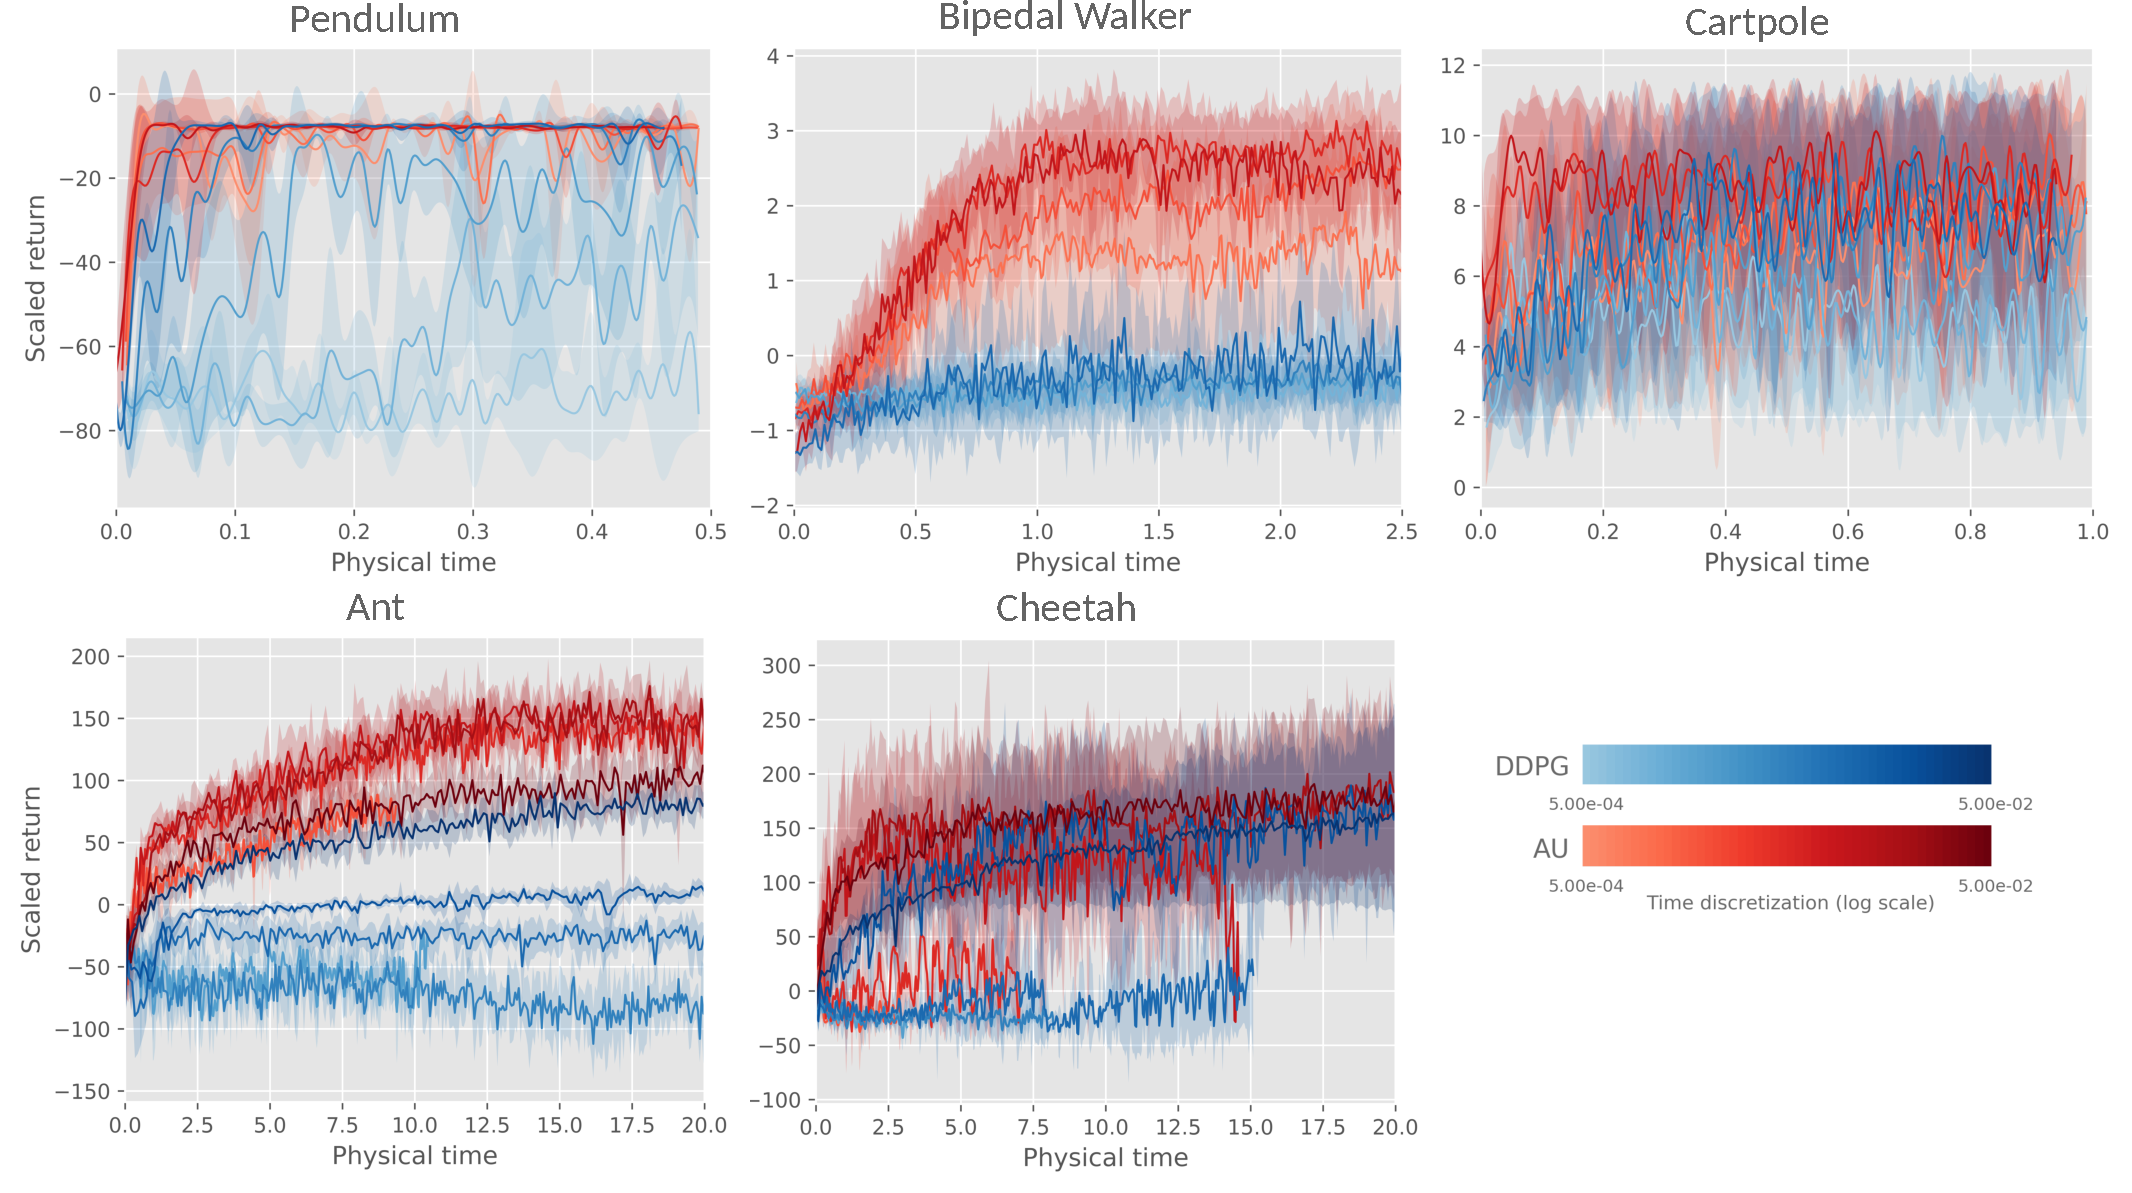
\includegraphics[width=\textwidth]{figs_data/full_results.pdf}
	\label{fig:full_results}
	\caption{Results on a variety of environments}
\end{figure*}

The experiments provided here are specifically aimed at showing that
the proposed method, DAU, works efficiently over a wide range of time
discretizations, without specific tuning, while standard deep $Q$-learning
approaches do not. DAU is compared to DDPG for continuous actions and to DQN
for discrete actions.  As mentionned earlier, we do not study the time
discretization invariance of on-policy methods (A3C, PPO, TRPO...).

In all setups, we use the algorithms described in
Alg.~\ref{alg:dau} and Supplementary Alg.~1. The variants of DDPG and DQN
used are described in the Supplementary, as well as all hyperparameters. We tested two different setups for DDPG and DQN.
In one, we scaled the discount factor (to avoid shortsightedness with small $\deltat$), but
left all other hyperparameters constant across time discretizations.
In the other, we used the properly rescaled discount
factor and reward from Eq.~\eqref{eq:def-gamma},
as well as $O(\deltat)$ learning rates for RMSProp.  The first variant yields slightly
better results, and is presented here, with the second variant in the
Supplementary. For all setups, quantitative results are averaged over five runs.

Let us stress that the quantities plotted are rescaled to make comparison
possible across different timesteps. For example,
returns are given in terms of the discretized return $R_\deltat$ as defined in \eqref{eq:discretized-return},\footnote{This mostly amounts to scaling rewards
by a factor $\deltat$ when this scaling is not naturally done in the environment. Environment-specific
details are given in the Supplementary.} and, most notably, time elapsed is always given in
\emph{physical} time, i.e., the amount of time that the agent spent
interacting with the environment (this is not the number of steps).


\paragraph{Qualitative experiments: Visualizing policies and values.}
To provide qualitative results, and check robustness to time
discretization both in terms of returns and in terms
of convergence of the approximate value function and policies, we first provide results on the simple pendulum environment
from the OpenAI Gym classic control suite.  The state space is of
dimension $2$. We visualize both the learnt value and policy functions by
plotting, for each point of the phase diagram $(\theta, \dot{\theta})$,
its value and policy. The results are presented in
Fig.~\ref{fig:pend} (value function) and Figs.~1, 2,  3 in
Supplementary.

We plot the learnt policy at several instants in physical time
during training, for various time discretizations
$\deltat$, for both DAU and DDPG. With DAU, the agent's policy and value
function quickly converge for every time discretization without specific
tuning. On the contrary, with DDPG, learning of both value function and
policy vary greatly from one discretization to another.

\paragraph{Quantitative experiments.}
We benchmark DAU against DDPG on classic control benchmarks: Pendulum,
Cartpole, BipedalWalker, Ant, and Half-Cheetah environments from OpenAI Gym. On
Pendulum, Bipedal Walker and Ant, DAU is quite robust to variations of
$\deltat$ and displays reasonable performance in all cases. On the other hand,
DDPG's performance varies with $\deltat$; performance either degrades as
$\deltat$ decreases (Ant, Cheetah), or becomes more variable as learning
progresses (Pendulum) for small $\deltat$. On Cartpole, noise dominates,
making interpretation difficult. On Half-Cheetah, DAU is not clearly
invariant to time discretization. This could be explained by the multiple
suboptimal regimes that coexist in the Half-Cheetah environment (walking on the
head, walking on the back), which create discontinuities in the value
function (see Discussion).
% \begin{figure}[h]
%   \centering
%   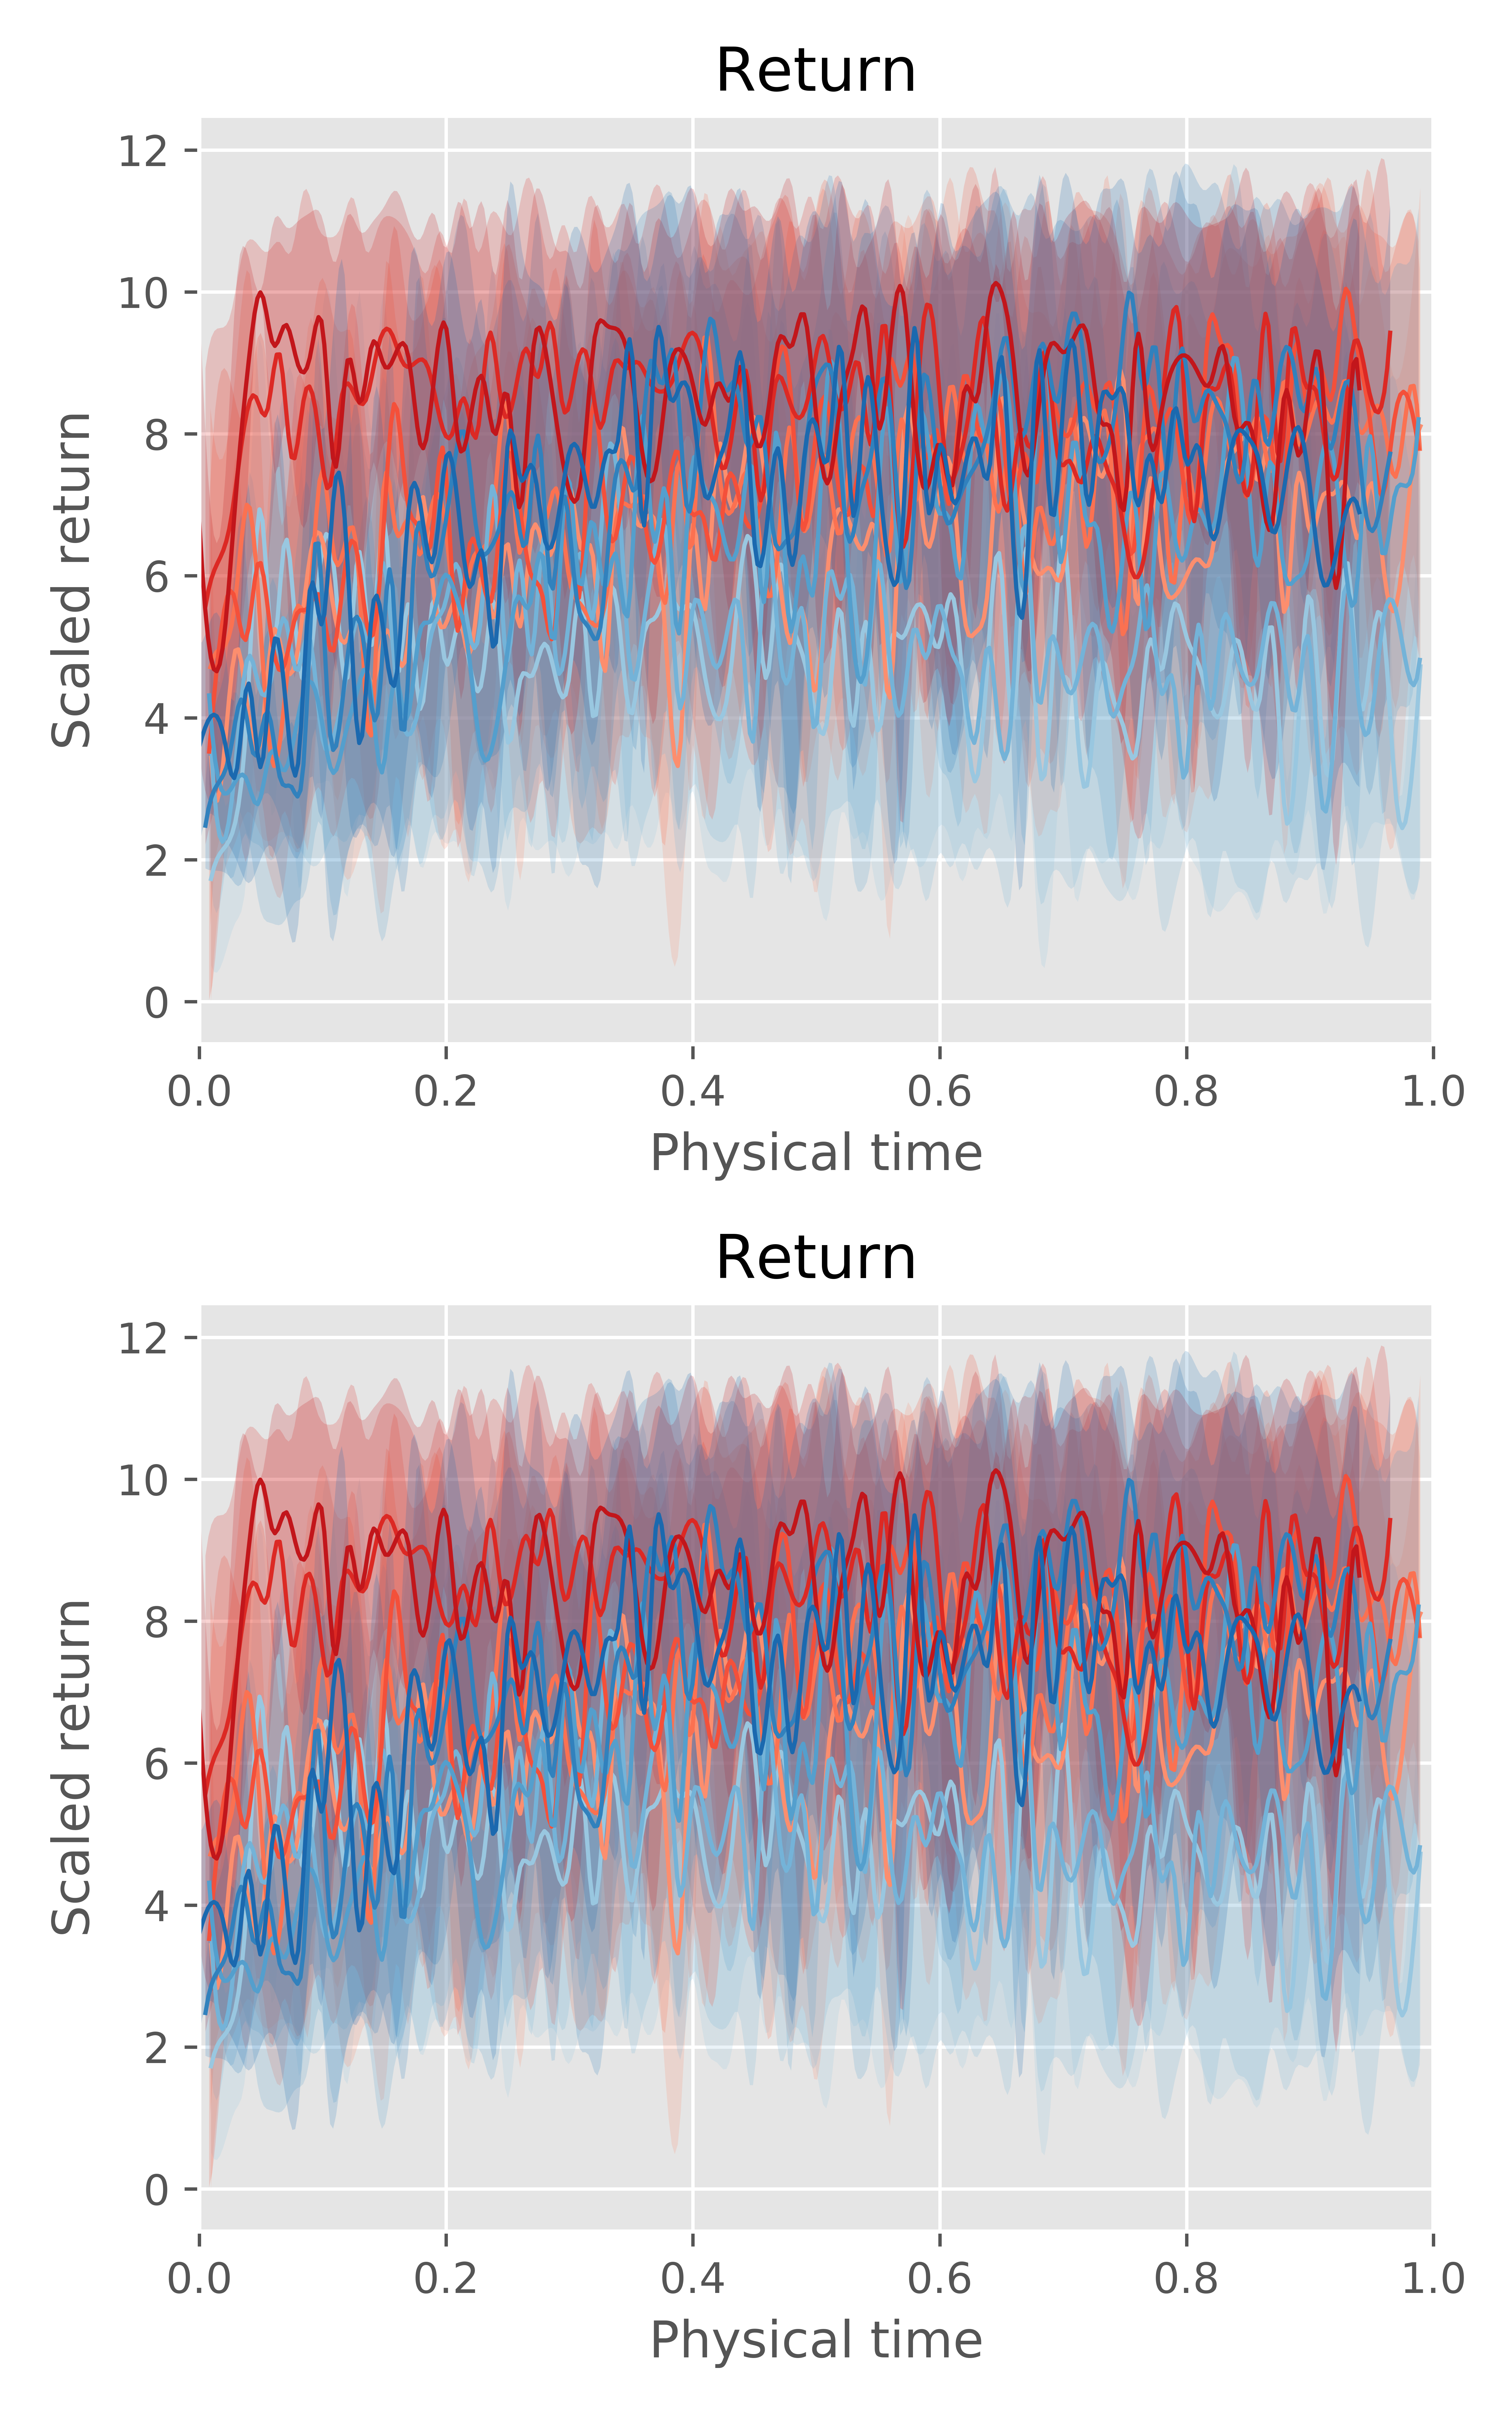
\includegraphics[width=\columnwidth]{figs_data/cartpole_lc.png}
%   \caption{Cartpole}
%   \label{fig:cartpole-lc}
% \end{figure}

% \begin{figure}[h]
%   \centering
%   \includegraphics[width=\columnwidth]{figs_data/ant_lc.png}
%   \caption{Ant}
%   \label{fig:ant-lc}
% \end{figure}
% 
% \begin{figure}[h]
%   \centering
%   \includegraphics[width=\columnwidth]{figs_data/pendulum_lc.png}
%   \caption{Pendulum}
%   \label{fig:pendulum-lc}
% \end{figure}


%%% Local Variables:
%%% TeX-master: "icml_drau"
%%% End:

%! TEX root = icml_drau.tex
\section{Discussion}
\label{sec:discussions}

The method derived in this work seems to yield improved robustness to
time discretization on various environments, e.g. pendulum swing up, or
simple locomotion tasks.  However on certain environments, there is still
room for improvment. In what follows, we identify some of the issues
that could explain this theoretical/practical discrepancy.

\paragraph{Smoothness of the value function.} In all of our proofs, $V^\pi$ is
assumed to be continuously differentiable for all $\pi$.  This %is a strong
hypothesis is not always satisfied in practice. 
\TODO{For instance, in the pendulum swing-up environment, depending on initial
position and momentum, the optimal policy needs to turn round a
certain number of times before reaching the target state. The value
function is discontinuous at the points of state space where the number
of turns changes.
% Very simple environments
% break this hypothesis, such as the pendulum swing-up environment,
% with pendulum height as reward and torque as action.  Indeed, 
% % assume that $\pi$
% % is the optimal policy for the pendulum swing-up environment, with state
% % representation $(\theta, \dot{\theta})$. 
% the state space $(\theta, \dot{\theta})$ for this environment
% can be partitioned into two subspaces $\mathcal{G}$ and $\mathcal{B}$, with
% $\mathcal{G}$ the subspace where the optimal policy 
% can swing up the pendulum without crossing the $y$-axis, and $\mathcal{B}$ where
% it has to cross the $y$-axis. The difference of $V$-function between a point in
% $\mathcal{G}$ and a point in $\mathcal{B}$ is lower bounded by a finite
% quantity. 
% %Besides, one can find two points $s_1 \in \mathcal{G}$ and $s_2 \in \mathcal{B}$
% %such that $s_1$ and $s_2$ are arbitrarily close.
% Consequently, the value function is
%discontinuous on the frontier between $\mathcal{G}$ and $\mathcal{B}$, which 
This results in non infinitesimal advantages
for actions on the boundary. In such environments where a given policy
has different regimes depending on the initial state, the continuous-time
analysis would only hold almost-everywhere.}
% more generally, as soon as a given policy has different regimes depending on
% where it starts in state space. For such policies the value
% function is typically discontinuous at the frontier between two
% regimes, resulting in non-infinitesimal advantages. The
% continuous-time DAU properties would only hold almost-everywhere.

\paragraph{Memory buffer size scalings}~Thm.~\ref{th:cont-params} is stated for
transitions sampled sequentially from a fixed trajectory. In practice,
transitions are sampled from a memory buffer, to prevent excessive correlations.
We used a fixed size circular buffer, filled
with samples from a single growing exploratory trajectory. In
our experiments, the same buffer size is used for all time discretizations. 
Thus the physical-time freshness of samples in the buffer varies with the
time discretization, and in the strictest sense using a fixed-size buffer
breaks timestep invariance. A memory-intensive option would be to use a
buffer of size $\frac{1}{\deltat}$ (fixed physical time); our theoretical
analysis does not cover this case.
% When
% $\deltat$ goes to $0$, this corresponds to learning nearly online on the
% infinite sequence, since the buffer will only contain examples that are very
% close temporally to the end of the sequence in physical time. \TODO{this
% contradicts the use of the buffer against correlations} While the resulting
% algorithm converges to a continuous time limit, in the strictest sense it is not
% time discretization invariant, as the freshness of samples in the buffer will
% vary with the time discretization.
% A different choice would be to scale the size of the buffer by a factor of
% $\frac{1}{\deltat}$. This would amount to always learning on the same physical time interval of
% the trajectory. Our theoretical analysis does not cover this case.
% \TODO{a bit too many details here?}

\paragraph{Near-continuous reinforcement learning and RMSProp.} RMSProp~\cite{rmsprop}
estimates a batched version of the second moment of gradients via moving
averages, and divides gradient steps by the square root of this estimate.
This may interact with the learning rate scaling discussed above. In
deterministic environments, gradients typically scale as $\bigO(1)$ in
term of $\deltat$, as seen in \eqref{eq:approx_bellman_A}.  In that case, RMSProp
preconditioning has no effect on the suitable order of magnitude for learning
rates. However, in near continuous \emph{stochastic} environments (Eq.~\ref{eq:sde}), variance of the gradients typically scales as
$\bigO\left(\frac{1}{\deltat}\right)$. With a fixed batch size,
RMSProp will multiply gradients by a factor $\bigO(\sqrt{\deltat})$. In
that case,
learning rates need only be scaled as $\alpha \,\sqrt{\deltat}$ instead of
$\alpha \,\deltat$.

More generally, the continuous-time analysis should in principle be repeated for every component of  
a system. For instance, if a recurrent model is used to handle state memory or partial observability, care should be taken that the model is able to maintain moemry for a non-infinitesimal physical-time when $\deltat\to 0$ (see for instance \TODO{chronornn}).

%! TEX root = icml_drau.tex
\section{Conclusion}

TODO



\pagebreak
\bibliography{icml_drau.bib}
\bibliographystyle{icml2019}
\end{document}


% This document was modified from the file originally made available by
% Pat Langley and Andrea Danyluk for ICML-2K. This version was created
% by Iain Murray in 2018. It was modified from a version from Dan Roy in
% 2017, which was based on a version from Lise Getoor and Tobias
% Scheffer, which was slightly modified from the 2010 version by
% Thorsten Joachims & Johannes Fuernkranz, slightly modified from the
% 2009 version by Kiri Wagstaff and Sam Roweis's 2008 version, which is
% slightly modified from Prasad Tadepalli's 2007 version which is a
% lightly changed version of the previous year's version by Andrew
% Moore, which was in turn edited from those of Kristian Kersting and
% Codrina Lauth. Alex Smola contributed to the algorithmic style files.

%%% Local Variables:
%%% TeX-master: "icml_drau"
%%% End:
